\chapter{ART Native Code Store}\label{chapter:native_code_store}

Since DEX code seems to be the vulnerable spot for Apps in terms of security
topics as well as for licensing and piracy issues, it makes sense to try
to circumvent this file format by design.
When comparing the mobile device distribution
system of Apps to desktop environments like Linux, Windows or MacOS, it becomes clear that the main difference is the distribution of Java like byte-code compared to binaries, at least for commercial software or the operating system itself. So the question would be if it is possible to establish an App store that only distributes native code instead of APKs. As derived in \autoref{section:app_execution_detail}, it is more than very likely that the DEX file is still needed for addressing native code inside of an ELF.
Nevertheless, that thought experiment will be performed in order to investigate if it would generally be possible.

At first, an architecture that would be suitable for an alternative native code App store needs to be defined. To keep the user experience as is, it would be beneficial to be able to still use the Google Play App Store for distributing Apps. Therefore at least a bare-bone APK for the application needs to be created that will then be placed into the Google Store.
That application can be installed the common Android way. At its first startup, it could connect to the actual native code App store
requesting the functional App in form of raw byte code or an ELF file that
somehow gets injected into the current bare-bone application.
Since the Android ODEX ELF file of an App has the DEX embedded, it would need to be adapted for instance leaving the DEX area blank.
So the skeleton version needs to implement at least the communication mechanism as well as the self modifying code part that can handle the receiving code snippets (\autoref{fig:native_store_arch} visually shows
the explained architecture).
\begin{figure}[htb]
  \centering
  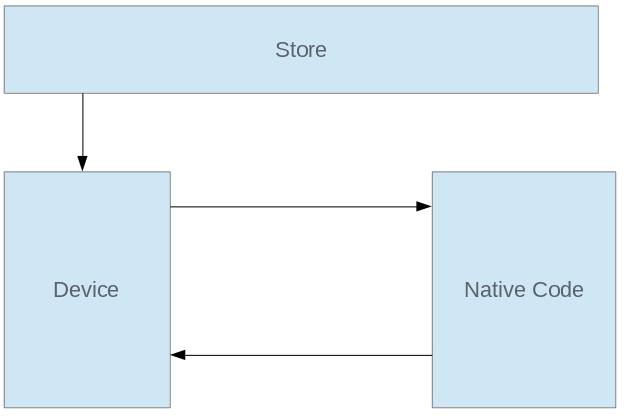
\includegraphics[scale=0.5]{figures/native_store_arch}
  \caption[Native Code Store Architecture]{Native Code Store Architecture}
  \label{fig:native_store_arch}
\end{figure}
When assuming that no root rights are present, the possibilities of injecting code and changing files are of course very limited. Remember that there exist two identical DEX files after the installation process (post Android 5), one DEX inside of the original \code{base.apk} package and one embedded inside the \code{dex2oat} output (ELF file).
Let's see to whom those files belong at Linux layer and what permissions are set. Files stored at \code{/data/app} like the \code{base.apk}, the \code{lib/}
folder as well as \code{oat/} belong to the \code{system} user. So accessing the \code{base.apk} container including its DEX should be
impossible from the App context without root rights. The same holds for the
\code{base.odex} which also belongs to \code{system} and is marked as
``\code{rw-}''.

Another way to check the possibilities of changing files dynamically at runtime are the mapped files and their permissions that can be read out of \code{/proc/self/maps} using C/C++ as explained in \autoref{section:memory_mapping}.
Remember that ``mapped'' means that those files are copied into the memory
and therefore changes made in mapped files are not taken over by the actual
physical stored counterparts. So changes written to mapped files would
not be permanent.
Since the last entity of an App getting executed is the ODEX file, it is
mapped into the process (\autoref{tab:app_odex_mapping} shows an example).
\begin{table}[htb]
  \caption[App's ODEX/ELF mapping]{App's ODEX/ELF mapping}
  \label{tab:app_odex_mapping}
  %\centering
  \texttt{
  \begin{tabular}{l l l l l l}
    \toprule
    address & perms & offset & dev & inode & rel. pathname \\
    \midrule
    a1d05000-a1fda000 & r--p & 00000000 & b3:1c & 171546 & app/.../oat/arm/base.odex \\
    a1fda000-a22ab000 & r-xp & 002d5000 & b3:1c & 171546 & app/.../oat/arm/base.odex \\
    a22ab000-a22ac000 & rw-p & 005a6000 & b3:1c & 171546 & app/.../oat/arm/base.odex \\
    a22ac000-a2327000 & r--p & 006ed000 & b3:1c & 171546 & app/.../oat/arm/base.odex \\
    \bottomrule
  \end{tabular}
  }
\end{table}
Several regions of the ODEX are mapped (offset marks the beginning relative to its file) with different permissions. Interesting is the part including writing permissions and its content. The corresponding ELF format was analyzed in \autoref{section:elf_file_format}. To find out which specific section is mapped as writable, a program can be written in order to dump the content of every section including its offset. Other options would be to just use a hex editor or even the \code{readelf} tool. So first, the ODEX has to be pulled out of the Android device for which root rights are required (otherwise it is not possible to even navigate into the App directory).
The file can then be moved into the \code{/sdcard} path and copied from a computer using \code{adb pull /sdcard/base.odex}. It then becomes clear that the mapped file region marked as writable is located in the string table section ``\code{.strtab}''. That mapped section though is not useful in terms of altering the Apps own code since it does not contain the DEX nor the ELF file. Therefore, a concept of distributing native code in form of cross-compiled ELF files without root rights is not possible.
